\documentclass{assignment}

\usepackage{float}
\usepackage{tikz}
\usepackage{adjustbox}
\usepackage{titlesec}
\usepackage{soul}
\usepackage{csvsimple}

\usepackage{bm}
\usepackage{amsmath,amssymb}

\usepackage{pgfplots}
\usepackage{graphics, epsfig}

\usepackage{graphicx}
\usepackage{subcaption}
\usepackage{matlab-prettifier}
\usepackage{multirow}

\usetikzlibrary{decorations.pathmorphing, decorations.markings}
\usetikzlibrary{positioning}

\usetikzlibrary{calc,patterns,angles,quotes}
\setlength{\parindent}{0pt}

\usetikzlibrary{shapes, arrows}
\tikzstyle{startstop} = [rectangle, rounded corners, minimum width=3cm, minimum height=1cm, text centered, draw=black, fill=red!30]
\tikzstyle{io} = [trapezium, trapezium stretches=true, trapezium left angle=70, trapezium right angle=110, minimum width=4cm, minimum height=1cm, text centered, draw=black, fill=blue!30]
\tikzstyle{process} = [rectangle, minimum width=4cm, minimum height=1cm, text centered, text width=4cm, draw=black, fill=orange!30]
\tikzstyle{decision} = [diamond, minimum width=3cm, minimum height=1cm, text centered, draw=black, fill=green!30]
\tikzstyle{arrow} = [thick,->,>=stealth]

\hypersetup{
pdftitle={Autonomous Vehicles},
pdfsubject={Assignment IV},
pdfauthor={Tommaso Bocchietti}
}

\makeglossaries

\begin{document}

\title{Autonomous Vehicles \\ Assignment IV: Algorithms for grid-based motion planning}
\author{Tommaso Bocchietti 10740309}
\date{A.Y. 2024/25}

\maketitle

\begin{figure}[H]
    \centering
    \includegraphics[width=0.7\textwidth]{./pdf/Polimi_logo_coverpage.pdf}
    \label{fig:Polimi_logo}
\end{figure}

\clearpage
\tableofcontents
\listoffigures
% \listoftables
% \lstlistoflistings
% \printglossary[type=\acronymtype]

\clearpage
\section{Introduction}
\label{sec:introduction}

The aim of this work is to gain insight into the development of a feedback control loop for an autonomous vehicle, specifically a \texttt{Turtlebot3} robot of the model \texttt{burger}.
Two different control strategies have been implemented, namely a simple proportional controller and a non-linear controller based on Lyapunov stability theory.
As for the simulation environment, the \texttt{Turtlebot3} robot was simulated in a Gazebo world, specifically the \texttt{turtlebot3\_world} provided by the \texttt{turtlebot3\_gazebo} package.

The following sections provide a detailed description of the requests associated with this assignment, the approach taken to fulfill them, and the discussion of the results obtained.

\paragraph{Tools}

As for the tools used, \texttt{ROS1} (Robot Operating System) is employed as the main framework for communication between the different components of the system.
\texttt{Simulink} is used as the main agent in the loop, sending control commands to the vehicles based on the telemetry data received from the vehicle itself.
\texttt{MATLAB} instead is used to perform the analysis of the data collected during the simulation, and to visualize the results.
Notice that with the current setup used by the author, \texttt{MATLAB 2024a} and \texttt{Simulink} are running in Windows 10, while \texttt{ROS1} is running in the \texttt{WSL2} (Windows Subsystem for Linux) environment, specifically in the \texttt{Ubuntu 22.04} distribution.

\section{Grid-based planning}
\label{sec:grid_based_planning}

In the field of robotics, a variety of algorithms are available for path planning, each with its own strengths and weaknesses.
One of the most ancient and well known class of algorithms is the so called \textit{Grid-based}, which is based on the discretization of the environment into a grid of cells.
Once the environment is represented as a grid, the problem of path planning is reduced to a graph search problem, where the cells of the grid are the nodes of the graph and the edges are the connections between adjacent cells.


\subsection{Requests}
\label{sec:requests}

Among the graph search algorithms, two of the most widely known are the \texttt{Dijkstra} and its extension \texttt{A*} algorithm.
The goal of this assignment can be summarized as follows:

\begin{itemize}
    \item Implement both the \texttt{Dijkstra} and \texttt{A*} algorithms;
    \item Allow the possibility of orthogonal and diagonal movements;
    \item Test the algorithms on a set of predefined maps and compare the performances.
\end{itemize}


\subsection{Graph search algorithms}
\label{sec:graph_search_algorithms}

In general, given a graph $G = (V, E)$, where $V$ is the set of vertices and $E$ is the set of edges, a graph search algorithm is used to find a path from a starting vertex $s \in V$ to a goal vertex $g \in V$.
The main idea is that the algorithm explores the graph by expanding nodes and evaluating their neighbors until it finds the goal node or exhausts all possibilities.

\begin{figure}[H]
    \centering

    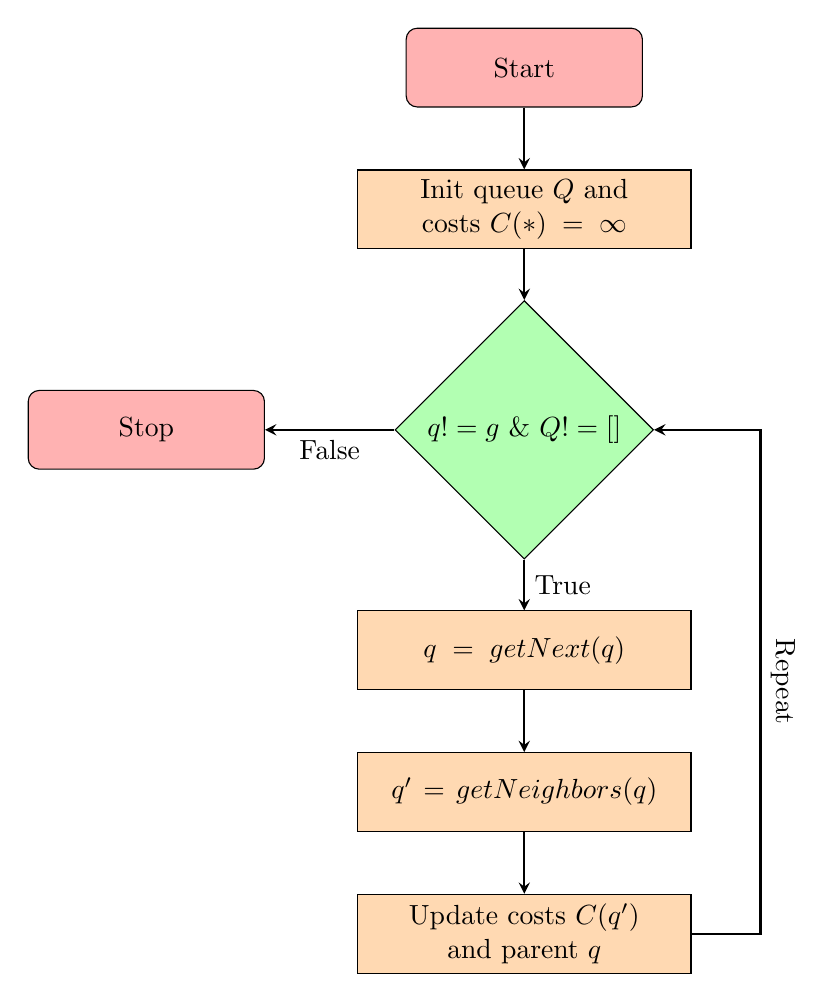
\begin{tikzpicture}[node distance=1.8cm]

        % Nodes
        \node (start) [startstop] {Start};
        \node (init) [process, below of=start] {Init queue $Q$ and costs $C(*) = \infty$};
        \node (check) [decision, below of=init, yshift=-1.0cm] {$q != g$ \& $Q != []$};
        \node (get_next) [process, below of=check, yshift=-1.0cm] {$q = getNext(q)$};
        \node (get_neighbors) [process, below of=get_next] {$q' = getNeighbors(q)$};
        \node (update) [process, below of=get_neighbors] {Update costs $C(q')$ and parent $q$};

        \node (stop) [startstop, left of=check, xshift=-3cm] {Stop};

        % Arrows
        \draw [arrow] (start) -- (init);
        \draw [arrow] (init) -- (check);
        \draw [arrow] (check) -- node[anchor=west] {True} (get_next);
        \draw [arrow] (get_next) -- (get_neighbors);
        \draw [arrow] (get_neighbors) -- (update);

        \draw [arrow] (update) -- +(3,0) |- (check.east) node[pos=0.25, above, rotate=-90] {Repeat};
        \draw [arrow] (check.west) -- node[anchor=north] {False} (stop);

    \end{tikzpicture}

    \caption{Generic graph search algorithm flowchart}
    \label{fig:graph_search_flowchart}

\end{figure}

The flowchart in Figure \ref{fig:graph_search_flowchart} summarizes the main steps of a generic graph search algorithm.
The algorithm starts by initializing the open list of nodes and the costs of all nodes to infinity.
Then, it enters a loop where based on the previous node visited, its neighbors are evaluated and added to the open list.
For each neighbor, the algorithm updates the cost if lower than what already stored and in case updates also the parent node.
The loop continues until the open list is empty, or the goal node is reached.

Grid-based algorithms have been proven to be complete and optimal, meaning that they will always find the shortest path if one exists.
However, they can be computationally expensive, especially in large environments.

There exist many variations built on top of the core algorithm presented in Figure \ref{fig:graph_search_flowchart}.
But, what really differentiates them, is the criteria used to select the next node to analyze from the open list.
Some of the most common approaches are:

\begin{itemize}
    \item \textbf{Depth-first search (DFS)}: explores as far as possible along each branch before backtracking. It uses a stack to keep track of the nodes to be explored. This approach can easily get stuck in loops.
    \item \textbf{Breadth-first search (BFS)}: explores all the neighbors of a node before moving on to the next level. It uses a queue to keep track of the nodes to be explored.
    \item \textbf{Best-first (a.k.a. Dijkstra)}: selects the node with the lowest cost from the start. This approach is optimal and complete, but can be slow in large environments.
    \item \textbf{A*}: an extension of Dijkstra's algorithm that uses a heuristic to estimate the cost from the current node to the goal node. This approach is also optimal and complete, and is often faster than Dijkstra's algorithm in practice, requiring a lower number of nodes to be explored.
\end{itemize}

In the following sections, we will focus on the Dijkstra and A* algorithms, explaining their mechanisms in choosing the next node to be explored and how they can be implemented to solve the path planning problem in a grid-based environment.



\subsubsection{Dijkstra's algorithm}
\label{sec:dijkstra_algorithm}

As already mentioned, Dijkstra's algorithm leverages the core structure of the graph search algorithm presented in Figure \ref{fig:graph_search_flowchart}, but with a specific strategy for selecting the next node to explore.

In particular, at each iteration, the algorithm selects the node among the nodes in the open list that has the lowest cost from the start node.
The idea is so to select $q' \in Q$ such that:

\begin{equation}
    q' = minarg_{q \in Q} C(q)
\end{equation}

Where $C(q)$ is the cost of reaching node $q$ from the start node $s$.
The cost is calculated as the sum of the cost of the previous node $q$ and the cost of moving from $q$ to $q'$.

From an implementation point of view, the algorithm can be easily implemented using a priority queue to store the nodes in the open list.
The priority queue allows for efficient retrieval of the node with the lowest cost, which is crucial for the performance of the algorithm.
Listing \ref{lst:dijkstra_algorithm} shows a possible implementation of the Dijkstra's algorithm.
The algorithm takes as input the graph $G$, the start node $s$, and the goal node $g$.

\begin{lstlisting}[
    style=Matlab-editor,
    caption={Code for the implementation of Dijkstra's algorithm.},
    label={lst:dijkstra_algorithm}
]
function [exist, distances, parents] = dijkstra(G, node_initial, node_final)
% DIJKSTRA Finds the shortest path between two nodes in a graph
% using Dijkstra's algorithm.

N = length(G.nodes);
distances = inf(N, 1);
parents   = NaN(N, 1);
visited   = false(N, 1);

% Initialization
ID_current = node_initial.ID;
distances(ID_current) = 0;

while (ID_current ~= node_final.ID && ~all(visited))

    unvisited = find(~visited);
    [~, ID_current] = min(distances(unvisited));
    ID_current = unvisited(ID_current);

    visited(ID_current) = true;

    % For each neighbor not yet visited
    IDs_neighbors = G.adjacents{ID_current};
    IDs_neighbors = IDs_neighbors(~visited(IDs_neighbors));
    for ID_neighbor = IDs_neighbors'

        distance = ...
            distances(ID_current) + ...
            G.getEdgeByConnection(ID_current, ID_neighbor).weight;

        if distance < distances(ID_neighbor)
            distances(ID_neighbor) = distance;
            parents(ID_neighbor) = ID_current;
        end

    end

end

exist = ~isinf(distances(node_final.ID));

end
\end{lstlisting}

The algorithm starts by initializing the distances of all nodes to infinity, except for the start node, which is set to zero.
Then, it enters a loop where it selects the node with the lowest cost from the open list and explores its neighbors.
For each neighbor, it updates the cost if the new cost is lower than the previously stored cost and updates the parent node accordingly.
The loop continues until the goal node is reached, or all nodes have been visited.
Finally, the algorithm returns the distances and parents of each node, which can be used to reconstruct the shortest path from the start node to the goal node.



\subsubsection{A* algorithm}
\label{sec:a_star_algorithm}

A* algorithm is an extension of Dijkstra's algorithm that uses a heuristic to estimate the cost from the current node to the goal node.
The heuristic is a function that provides an estimate of the cost to reach the goal from a given node, and it is used to guide the search towards the goal more efficiently.

In particular, the A* algorithm selects the next node to explore based on the sum of the cost from the start node to the next node and the estimated cost from the next node to the goal node.
The selection is done as follows:

\begin{equation}
    q' = min\arg_{q \in Q} (C(q) + h(q))
\end{equation}

Where $h(q)$ is the heuristic function that estimates the cost from node $q$ to the goal node $g$.
The heuristic function can be any function that provides an estimate of the cost, but it is important that it is admissible, meaning that it never overestimates the true cost to reach the goal.
For the sake of simplicity, and in particular leveraging the meaningful geometrical interpretation of the grid-based environment, we will use the Euclidean distance as the heuristic function.
The A* algorithm can be implemented similarly to Dijkstra's algorithm, with the addition of the heuristic function.
Listing \ref{lst:a_star_algorithm} shows a possible implementation of the A* algorithm.
The algorithm takes in the same input as the Dijkstra's one.

\begin{lstlisting}[
    style=Matlab-editor,
    caption={Code for the implementation of A* algorithm.},
    label={lst:a_star_algorithm}
]
function [exist, distances, parents] = astar(G, node_initial, node_final)
% ASTAR Finds the shortest path between two nodes in a graph
% using the A* algorithm.

N = length(G.nodes);
distances = inf(N, 1);
costs     = inf(N, 1);
parents   = NaN(N, 1);
visited   = false(N, 1);

% Initialization
ID_current = node_initial.ID;
distances(ID_current) = 0;
costs(ID_current) = Node.euclideanDistance(node_initial.state, node_final.state);

while (ID_current ~= node_final.ID && ~all(visited))

    unvisited = find(~visited);
    [~, ID_current] = min(costs(unvisited));
    ID_current = unvisited(ID_current);

    visited(ID_current) = true;

    % For each neighbor not yet visited
    IDs_neighbors = G.adjacents{ID_current};
    IDs_neighbors = IDs_neighbors(~visited(IDs_neighbors));
    for ID_neighbor = IDs_neighbors'

        distance = ...
            distances(ID_current) + ...
            G.getEdgeByConnection(ID_current, ID_neighbor).weight;

        if distance < distances(ID_neighbor)

            distances(ID_neighbor) = distance;
            parents(ID_neighbor) = ID_current;

            node_neighbor = G.getNodeByID(ID_neighbor);
            costs(ID_neighbor) = distance + Node.euclideanDistance(node_neighbor.state, node_final.state);

        end

    end

end

exist = ~isinf(distances(node_final.ID));

end
\end{lstlisting}

One can clearly notice that the structure of the A* algorithm is basically the same as the Dijkstra's algorithm, except for the addition of the heuristic function in the cost calculation.
Notice also that the heuristic function is only used to update the cost of the nodes in the open list, and it is not used to update the distances of the nodes from the start node.

Given that now the algorithms is somehow guided, one can expect that the A* algorithm will be faster than the Dijkstra one, as fewer nodes will be explored.
\section{Algorithm Testing}
\label{sec:algorithm_testing}

Now that the algorithm has been implemented, we can proceed presenting at first the test environment that have been used to test them and then the results of the tests.

Figures \ref{fig:test_maps} show the four image maps used to test the algorithm.
Even if the images here below are of size 300x300, we preferred to scale down to 30x30 given that each pixel is then converted into a node of the graph and so to avoid huge graphs and long computation times.
Notice also that while the white areas are free space, the one marked in black or gray are to be considered as obstacles.
Finally, the green dot is the starting point of the vehicle, while the red one is the goal.

\begin{figure}[H]
    \centering
    \frame{\includegraphics[width=0.48\textwidth]{./img/01.png}}
    \hspace{6pt}
    \frame{\includegraphics[width=0.48\textwidth]{./img/02.png}}

    \vspace{11pt}

    \frame{\includegraphics[width=0.48\textwidth]{./img/03.png}}
    \hspace{6pt}
    \frame{\includegraphics[width=0.48\textwidth]{./img/04.png}}
    \caption{Test maps used for the algorithm testing.}
    \label{fig:test_maps}
\end{figure}

In the following, results obtained running both the A* and the Dijkstra algorithms on each of the four maps are presented.

The plotting of both the (geometrical) connected graph and the best path found is also shown.
Notice that each test case has been run allowing or disabling the diagonal movement of the vehicle, which can be achieved during the graph generation phase modifying the connection of the nodes.

Tables presenting the main metrics of the tests are also shown.
The metrics are the following:

\begin{itemize}
    \item \textbf{Elapsed time}: here only the time needed to run the searching algorithm is considered (i.e. we are excluding both the generation of the graph and the plotting of the results);
    \item \textbf{Nodes analyzed}: number of nodes analyzed (visited) before reaching the goal;
    \item \textbf{Path length}: length of the path found by the algorithm. This also correspond to the path cost, given that the cost of each edge is equal to its geometrical length.
\end{itemize}



\subsection{Map 1}
\label{subsec:map_1}

Results obtained running the A* and Dijkstra algorithms on Map 1 are shown in Figures \ref{fig:map_1_results} and Table \ref{tab:map_1_results}.
About the figures, the upper row shows the graph generated running the Dijkstra algorithm while the lower one shows the graph generated running the A* algorithm.
The left column shows the graph generated allowing only orthogonal movements, while the right one shows the graph generated allowing also diagonal movements.
The path found by the algorithm is shown in red, while the graph is shown in black.

\begin{figure}[H]
    \centering
    \includegraphics[width=0.48\textwidth]{./img/MATLAB/01_dijkstra_orthogonal.pdf}
    \hspace{6pt}
    \includegraphics[width=0.48\textwidth]{./img/MATLAB/01_dijkstra_diagonal.pdf}

    \vspace{11pt}

    \includegraphics[width=0.48\textwidth]{./img/MATLAB/01_astar_orthogonal.pdf}
    \hspace{6pt}
    \includegraphics[width=0.48\textwidth]{./img/MATLAB/01_astar_diagonal.pdf}
    \caption{Map 1: Graph and path found by the algorithms.}
    \label{fig:map_1_results}
\end{figure}

\begin{table}[H]
    \centering
    \begin{tabular}{|c|c|c|c|c|c|}
        \hline
        \textbf{Algorithm}        & \textbf{Diagonal} & \textbf{Elapsed time (ms)} & \textbf{Nodes analyzed} & \textbf{Path length (m)} \\
        \hline
        \multirow{2}{*}{Dijkstra} & No                & 624                        & 456                     & 53                       \\
                                  & Yes               & 1592                       & 453                     & 47                       \\
        \hline
        \multirow{2}{*}{A*}       & No                & 339                        & 378                     & 53                       \\
                                  & Yes               & 1227                       & 339                     & 47                       \\
        \hline
    \end{tabular}
    \caption{Map 1: Results of the tests.}
    \label{tab:map_1_results}
\end{table}

From the results presented in Table \ref{tab:map_1_results} and in Figure \ref{fig:map_1_results}, we can already notice that while the cost of the path found by the two algorithms is equivalent, the number of nodes considered by the A* algorithm is significantly lower than the one considered by the Dijkstra algorithm.
This behavior is expected due to the use of the heuristic function to guide the search of the A* algorithm.
The advantage in terms of computational time is also evident, with the A* algorithm outperforming the Dijkstra algorithm.



\subsection{Map 2}
\label{subsec:map_2}

Results obtained running the A* and Dijkstra algorithms on Map 2 are shown in Figures \ref{fig:map_2_results} and Table \ref{tab:map_2_results}.
The same layout of the previous map is used for the figures and the same metrics are used for the table.

\begin{figure}[H]
    \centering
    \includegraphics[width=0.48\textwidth]{./img/MATLAB/02_dijkstra_orthogonal.pdf}
    \hspace{6pt}
    \includegraphics[width=0.48\textwidth]{./img/MATLAB/02_dijkstra_diagonal.pdf}

    \vspace{11pt}

    \includegraphics[width=0.48\textwidth]{./img/MATLAB/02_astar_orthogonal.pdf}
    \hspace{6pt}
    \includegraphics[width=0.48\textwidth]{./img/MATLAB/02_astar_diagonal.pdf}
    \caption{Map 2: Graph and path found by the algorithms.}
    \label{fig:map_2_results}
\end{figure}

\begin{table}[H]
    \centering
    \begin{tabular}{|c|c|c|c|c|c|}
        \hline
        \textbf{Algorithm}        & \textbf{Diagonal} & \textbf{Elapsed time (ms)} & \textbf{Nodes analyzed} & \textbf{Path length (m)} \\
        \hline
        \multirow{2}{*}{Dijkstra} & No                & 1009                       & 731                     & 46                       \\
                                  & Yes               & 3963                       & 742                     & 37                       \\
        \hline
        \multirow{2}{*}{A*}       & No                & 732                        & 490                     & 46                       \\
                                  & Yes               & 1434                       & 233                     & 37                       \\
        \hline
    \end{tabular}
    \caption{Map 2: Results of the tests.}
    \label{tab:map_2_results}
\end{table}

Similarly to the previous map, the results presented in Table \ref{tab:map_2_results} and in Figure \ref{fig:map_2_results} show that while the cost of the path found by the two algorithms is equivalent, the number of nodes considered by the A* algorithm is significantly lower than the one considered by the Dijkstra algorithm.
Similar conclusions can be drawn in terms of computational time and performance of the two algorithms.

As an additional note, in this case we can also appreciate that the number of analyzed nodes by A* is significantly lower than the one analyzed by Dijkstra, particularly in case of diagonal movements.
This is, however, expected.
Looking at the final path, we observe that is almost equivalent to the diagonal connecting ideally the start and goal points.
This means that the heuristic function used by A* is even more effective in this case, given that very few obstacles are present along the optimal path designed by the heuristic function itself and so fewer death ends are encountered.
In other words, if the optimal path turns out to be a straight line connecting the start and goal points, the A* algorithm would analyze a number of nodes equal to the number of nodes along the straight line, while the Dijkstra algorithm would still analyze a much larger number of nodes given that no information is used to guide the search.


\subsection{Map 3}
\label{subsec:map_3}

Results obtained running the A* and Dijkstra algorithms on Map 3 are shown in Figures \ref{fig:map_3_results} and table.
The same layout of the previous map is used for the figures and the same metrics are used for the table.

\begin{figure}[H]
    \centering
    \includegraphics[width=0.48\textwidth]{./img/MATLAB/03_dijkstra_orthogonal.pdf}
    \hspace{6pt}
    \includegraphics[width=0.48\textwidth]{./img/MATLAB/03_dijkstra_diagonal.pdf}

    \vspace{11pt}

    \includegraphics[width=0.48\textwidth]{./img/MATLAB/03_astar_orthogonal.pdf}
    \hspace{6pt}
    \includegraphics[width=0.48\textwidth]{./img/MATLAB/03_astar_diagonal.pdf}
    \caption{Map 3: Graph and path found by the algorithms.}
    \label{fig:map_3_results}
\end{figure}

\begin{table}[H]
    \centering
    \begin{tabular}{|c|c|c|c|c|c|}
        \hline
        \textbf{Algorithm}        & \textbf{Diagonal} & \textbf{Elapsed time (ms)} & \textbf{Nodes analyzed} & \textbf{Path length (m)} \\
        \hline
        \multirow{2}{*}{Dijkstra} & No                & 567                        & 592                     & 87                       \\
                                  & Yes               & 2461                       & 592                     & 74                       \\
        \hline
        \multirow{2}{*}{A*}       & No                & 496                        & 497                     & 87                       \\
                                  & Yes               & 1780                       & 452                     & 74                       \\
        \hline
    \end{tabular}
    \caption{Map 3: Results of the tests.}
    \label{tab:map_3_results}
\end{table}

Again, similar considerations as before can be drawn from the results presented in Table \ref{tab:map_3_results} and in Figure \ref{fig:map_3_results}.


\subsection{Map 4}
\label{subsec:map_4}

Results obtained running the A* and Dijkstra algorithms on Map 4 are shown in Figures \ref{fig:map_4_results} and table.
The same layout of the previous map is used for the figures and the same metrics are used for the table.

\begin{figure}[H]
    \centering
    \includegraphics[width=0.48\textwidth]{./img/MATLAB/04_dijkstra_orthogonal.pdf}
    \hspace{6pt}
    \includegraphics[width=0.48\textwidth]{./img/MATLAB/04_dijkstra_diagonal.pdf}

    \vspace{11pt}

    \includegraphics[width=0.48\textwidth]{./img/MATLAB/04_astar_orthogonal.pdf}
    \hspace{6pt}
    \includegraphics[width=0.48\textwidth]{./img/MATLAB/04_astar_diagonal.pdf}
    \caption{Map 4: Graph and path found by the algorithms.}
    \label{fig:map_4_results}
\end{figure}

\begin{table}[H]
    \centering
    \begin{tabular}{|c|c|c|c|c|c|}
        \hline
        \textbf{Algorithm}        & \textbf{Diagonal} & \textbf{Elapsed time (ms)} & \textbf{Nodes analyzed} & \textbf{Path length (m)} \\
        \hline
        \multirow{2}{*}{Dijkstra} & No                & 725                        & 650                     & 55                       \\
                                  & Yes               & 2799                       & 650                     & 47                       \\
        \hline
        \multirow{2}{*}{A*}       & No                & 640                        & 562                     & 55                       \\
                                  & Yes               & 2060                       & 450                     & 47                       \\
        \hline
    \end{tabular}
    \caption{Map 4: Results of the tests.}
    \label{tab:map_4_results}
\end{table}

Once again, even from the tests on Map 4, similar conclusions as before can be drawn from the results presented in Table \ref{tab:map_4_results} and in Figure \ref{fig:map_4_results}.


\section{Conclusions}
\label{sec:conclusions}

In this short report, we have presented the results of the first assignment of the course on Autonomous Vehicles.
We have shown how to analyze data collected by a simulated robot in a Gazebo environment, using the \texttt{rosbag} command to store the data.
We have also demonstrated how to estimate the control commands sent to the robot during the simulation, and how to evaluate their accuracy by comparing trajectories and odometer readings.

Results obtained show that the estimated commands are representative of the original ones, but not completely overlapping due to poor timing performance caused (probably) by the \texttt{WSL2} environment that can't fully afford the real-time performance required by the simulation.

Further investigations and testing could be done by switching to a native \texttt{Linux} environment, which could provide better performance and more accurate results.

% \vspace*{\fill}
% \nocite{*}
% \bibliographystyle{plain}
% \bibliography{references.bib}

\clearpage
\appendix
\section{MATLAB Graph implementation}
\label{sec:graph_implementation}

During the implementation of the Dijkstra and A* algorithms, a needs for a solid and efficient graph representation arose.
In order to achieve this, a set of MATLAB classes was created to represent the graph, its nodes and its edges.

In the following, the complete code used for this purpose is shown.
One can refer back to the graph search algorithm implementation to understand how these classes are used.

\lstinputlisting[
    style=Matlab-editor,
    caption={Graph class used to represent a weighted and directed/undirected graph.}
]{files/Graph.m}

\lstinputlisting[
    style=Matlab-editor,
    caption={Edge class used to represent a weighted and directed edge in the graph.}
]{files/Edge.m}

\lstinputlisting[
    style=Matlab-editor,
    caption={Node class used to represent a node in the graph.}
]{files/Node.m}


As a final note, a code profiler was used to test the performance of the graph implementation.
The main bottleneck was found in the \texttt{getEdgeByConnection} method of the \texttt{Graph} class, as shown in Figure \ref{fig:graph_profiler}.

\begin{figure}[H]
    \centering
    \includegraphics[width=1.0\textwidth]{./img/code_profile.png}
    \caption{Profiler output for the graph implementation.}
    \label{fig:graph_profiler}
\end{figure}

The author of this report is aware that the graph implementation can be improved in terms of performance by using perhaps a caching mechanism or a more efficient data structure.
However, this was not the main focus of the assignment and further investigation is left as future work.


\end{document}
